%!TEX encoding = UTF-8 Unicode

%----------------------------------------------------------------------------------------
%   CHAPTER 9
%   translator: inempty, 不变态的海森堡
%   proofreader: inempty, SI
%----------------------------------------------------------------------------------------

\chapterimage{chapter_head_1.pdf}

\chapter[量子场论]{Quantum Field Theory \quad 量子场论}
\label{chap9}

\section*{总结\, \sout{剧透}}
{\it 译注:本节的内容是介绍本章将要做些什么\sout{也就是剧透},第一遍读不懂属于正常情况。}

本章介绍量子场论的基本框架。由第\ref{chap5}章导出的公式
$$ [\Phi(x), \pi(y)] = i \delta(x - y) $$
可见场本身就是算符。自旋为$0, 1/2, 1$的场的运动方程的解是用场的{\bf Fourier展开}\mpar{Fourier变换背后的思想在附录D.1中进行了解释.}写出来的。从上式的对易关系可见Fourier系数也是算符。之后,我们会看到这些{\bf 算符}(当然还包括导出它们的场)是如何{\bf 产生和湮灭粒子}的,用对应场的拉格朗日量可以导出代表能量的哈密顿算符。

之后建立{\bf 相互作用理论},它是量子场论的核心。 我们会看到在相互作用理论中,哈密顿量是由自由场的哈密顿量和{\bf 相互作用的哈密顿量}线性组合而成的。这一思路之后可应用于{\bf 相互作用绘景}中,在这个绘景下场的时间演化是由自由哈密顿量主导的,而态的时间演化是由相互作用哈密顿量主导的。在这个绘景下,能够推导出散射过程的几率幅,用Dirac记号可以表示成
$$\langle f | \hat{S} | i\rangle,$$

这里$\hat{S}$表示描述散射过程的算符,$|i\rangle$是初态,$\langle f|$是末态。 我们会发现算子$\hat{S}$可以用相互作用哈密顿量$H_{I}$写成
$$\hat{S}(t,t_{i}) = \mathrm{e}^{-i\int_{t_{i}}^{t} dt' H_{I}}.$$

这个式子解不出来,因此采用级数展开式来计算这个指数。对于大多数实验而言,前面几项就足以精确的描述了。

级数展开中的每一项可以解释为描述不同种类的散射过程。相互作用哈密顿量包含了场的线性组合,就如上面提到的,是用来产生或者湮灭场的。对于最低的非平凡阶次,我们得到8项,且第一项描述了一个从$e^{-} e^{+} \to \gamma$的散射过程。这意味着我们从一个由电子和正电子组成的初态$|e^{-}e^{+} \rangle$出发,这个初态被自旋1/2的场算符湮灭,并且之后一个光子$\langle \gamma |$由光子场产生。其他项作用在初态$|e^{-}e^{+} \rangle$时的结果是0。

这个级数的下一阶由许多项组成,我们只考虑其中的一项,同样地,从初态$|e^{-}e^{+} \rangle$开始,其中的一项描述了过程$e^{-}e^{+} \to \gamma \to e^{-}e^{+}$, 这里初末的正负电子对一般具有不同的动量。

同样地,所有这些项可以理解成所有的相互作用哈密顿量。一种简化这类计算的图形化方法是著名的Feynman图。在这个图中每一条线,每一个顶点代表了上面计算的东西的一个因子。

\section[对应到场理论]{Field Theory Identifications \quad 对应到场理论}
\label{sec9.1}
本节探究从对称性限制得到的拉格朗日量是怎样应用到场论的框架中的。要得到一个描述自然界的场论,第一步是将拉格朗日量和第\ref{chap5}章内容,尤其是\eqref{equ5.5}式\footnote{译注:似乎应该为\eqref{eq5.6}式。}结合起来,为了方便,将\eqref{equ5.5}式重写一遍:
\begin{equation}
\label{equ9.1}
    [\Phi(x), \pi(y)] = i\delta(x - y)
\end{equation}
其中共轭动量密度$\pi(y)$为
\begin{equation}
\label{equ9.2}
    \pi(y)=\frac{\partial \mathscr{L}}{\partial(\partial_{0}\Phi(y))}
\end{equation}
\section[自旋为$0$的自由场理论]{Free Spin 0 Field Theory \quad 自旋为$0$的自由场理论}
\label{sec9.2}
{\small “一个产生的艺术首先是一个毁灭的艺术。”\\\rightline{——{\bf Pablo Picasso}}}\mpar{引自Rollo May,\textit{The Courage to Create}. W.W.Norton and Company,reprint edition,3 1994. ISBN 9780393311068}

从最简单的例子——自由的$0$自旋场——出发,它由在Lorentz变换下不变的标量来描述(在\ref{sec3.7.4}节推导)。我们已经在\ref{sec6.2}节中推出了相对应的拉格朗日量\footnote{原文下式有误,译文已按勘误表修改。}
\begin{equation} \label{equ9.3}
    \mathscr{L}=\frac{1}{2}(\partial_{\mu}\Phi \partial^{\mu}\Phi-m^{2}\Phi^{2})
\end{equation}
它的运动方程叫做Klein-Gordon方程
\begin{equation} \label{equ9.4}
    (\partial_{\mu}\partial^{\mu}+m^{2})\Phi=0
\end{equation}
可直接计算出共轭动量
\[
    \pi(x)=\frac{\partial \mathscr{L}}{\partial( \partial_{0}\Phi(x))}=\frac{\partial}{\partial(\partial_{0}\Phi(x))} \frac{1}{2} \Big(\partial_{\mu}\Phi(x)\partial^{\mu}\Phi(x)-m^{2}\Phi^{2}(x) \Big) = \partial_{0}\Phi(x)
\]
Klein-Gordon方程的最一般的解可以写成Fourier展开的形式\mpar{如果想知道关于积分测度的详细的计算过程,以及为什么写出这种形式的解的验证请看本章最后\ref{sec9.6}的附录。}
\begin{equation} \label{equ9.5}
	\Phi(x)=\int dk^{3}\, \frac{1}{(2\pi)^{3}2\omega_{k}} \big( a(k) e^{-ikx} + b(k) e^{ikx} \big)
\end{equation}
其中\footnote{原文此式有误,译文已按勘误表修改。}$\omega_k^{2} \equiv \vec{k}^{2} + m^{2}$,如果限制在实标量场的情况上式可写为
\begin{equation} \label{equ9.6}
	\Phi(x)=\int dk^{3}\, \frac{1}{(2\pi)^{3}2\omega_{k}} \big( a(k)e^{-ikx}+a^{\dag}(k)e^{ikx} \big)
\end{equation}
因为$c+c^{\dag}=\underbrace{\text{Re}(c)+i \cdot \text{Im}(c)}_{c}+\underbrace{\text{Re}(c)-i \cdot \text{Im}(c)}_{c^{\dag}}=2\text{Re}(c)$.

现在考虑方程\eqref{equ9.1},即不为零的对易子$[\Phi(x),\pi(y)]\neq 0$有什么含义。这意味着$\Phi(x)$和$\pi(y)$不是普通的函数而必须是算符,因为一般的函数是对易的:$(3+x)(7xy)=(7xy)(3+x)$。由方程\eqref{equ9.6}可以得到结论:Fourier系数$a(k)$和$a(k)^{\dag}$是算符,因为$e^{\pm ikx}$只是复数,而复数是对易的。

从方程\eqref{equ9.1}可以计算出\mpar{例如可以参考Lewis H.Ryder书的4.1节,{\it Quantum Field Theory}. Cambridge University Press, 2nd edition, 6 1996. ISBN 9780521478114}
\begin{align}
	[a(k),a^{\dag}(k')]=(2\pi)^{3}\delta^{3}(\vec{k}-\vec{k'}) \label{equ9.7} \\
	[a(k),a(k')]=0 \label{equ9.8} \\
	[a^{\dag}(k),a^{\dag}(k')]=0 \label{equ9.9}
\end{align}
既然已经知道场就是算符,接下来自然要问:{\bf 它作用在什么上面?}在粒子理论中,动力学变量与算符相等同,算符作用的数学对象(波函数,抽象的Dirac右矢等等)描述粒子。在场论中,目前没有什么东西来描述粒子。在这一点上,粒子是怎么出现在场论中是完全不清楚的。然而,通过考虑场的展开系数$a(k)$和$a^{\dag}(k)$作用于什么抽象的数学对象上,就可以知道场作用在什么对象上的了。为了建立直观认识,我们从熟悉的能量入手。

一个标量场的能量$E$由时间平移不变性导出的方程\eqref{equ4.40}给出:
\begin{align}
	E &= \int d^{3}x T^{00} \notag \\
	&= \int d^{3}x \left(\frac{\partial \mathscr{L}}{\partial(\partial_{0}\Phi)}\underbrace{\frac{\partial \Phi}{\partial x_{0}}}_{\partial_{0}\Phi}-\mathscr{L} \right) \notag \\
	&= \int d^{3}x \left( \partial_{0}\Phi)^{2} - \frac{1}{2}(\partial_{\mu}\Phi \partial^{\mu}\Phi-m^{2}\Phi^{2} \right) \notag \\
	&\underbrace{=}_{ \mathclap{ \partial_{\mu}\partial^{\mu}=\partial_{0} \partial_{0}-\partial_{i}\partial_{i} } } \frac{1}{2}\int d^{3}x \Big( (\partial_{0}\Phi)^{2}+(\partial_{i}\Phi)^{2}+m^{2}\Phi^{2} \Big) \label{equ9.10}
\end{align}
将方程\eqref{equ9.6}代入方程\eqref{equ9.10},并利用对易关系$\eqref{equ9.7} \sim \eqref{equ9.9}$式可得
\begin{align}
	E &= \frac{1}{2} \int dk^{3}\, \frac{1}{(2\pi)^{3}} \omega_{k} \Big( a^{\dag}(k)a(k)+a(k)a^{\dag}(k) \Big) \nonumber\\ 
	&\underbrace{=}_{\mathclap{\ref{equ9.7}\text{式} } } \int dk^{3}\,\frac{1}{(2\pi)^{3}} \omega_{k} \left( a^{\dag}(k)a(k)+\frac{1}{2}(2\pi)^{3}\delta^{3}(0) \right) \label{equ9.11}
\end{align}
这时我们的理论发散了,积分中的第二项是无穷大的。我们可以在这里停下并且说这个理论无效。然而,一些勇敢的人进行了深入的探索,忽略无穷大项并且发现了一个精确描述自然的理论。从这里继续的标准的做法就是忽略第二项,这种做法的可行性尚未得到解释。不过这里的关键在于发散项出现在每个系统的能量中,并且我们只能测量能量的差值。因此这个无穷大的常数项不会对测量造成影响。

按照习惯,写作算符的能量叫做哈密顿量$\hat{H}$, 我们可以计算$\hat{H}$和Fourier系数$a(k)$以及$a^{\dag}(k)$的对易子\mpar{之后会看到它有什么用。}。我们得到了
\begin{align}
	[\hat{H},a^{\dag}(k')] &= \int dk^{3}\, \frac{1}{(2\pi)^{3}} \omega_{k}[a^{\dag}(k)a(k),a^{\dag}(k')]\nonumber\\
	&\underbrace{=}_{\mathclap{[a^{\dag}(k),a^{\dag}(k')]=0}} \int dk^{3}\,\frac{1}{(2\pi)^{3}} \omega_{k} a^{\dag}(k) [a(k),a^{\dag}(k')]\nonumber\\
	&=\int dk^{3}\,\omega_{k}a^{\dag}(k)\delta^{3}(k-k')\nonumber\\
	&\underbrace{=}_{ \mathclap{\text{见附录D.2}}} \omega_{k'}a^{\dag}(k') \label{equ9.12}
\end{align}
同样的
\begin{equation}
\label{equ9.13}
	[\hat{H}, a(k')] = -\omega_{k'} a(k')
\end{equation}
量子理论中的算符作用于描述系统状态的数学对象上(见\ref{sec8.3}节)。在这个情况下,如果用能量算符,即哈密顿算符$\hat{H}$作用在抽象的对象$| ? \rangle$上来描述物理系统,就能得到系统的能量:
\begin{equation} \label{equ9.14}
	\hat{H} |?\rangle=E | ?\rangle
\end{equation}
现在回到开始的那个问题:{\bf 场\mpar{记住:场=算符}是如何作用于物理系统的?}先来考虑\mpar{这里我们采取了非常聪明的处理方式,它是Dirac在处理量子力学中谐振子的问题时首先被引入的}第一个Fourier系数(它是个算符)对于系统能量的影响:
\begin{align}
	\hat{H} \Big( a(k')| ?\rangle \Big) &= \Big( a(k')\hat{H} + \underbrace{\hat{H}a(k')-a(k')\hat{H}}_{[\hat{H},a(k')]} \Big) |?\rangle \notag \\
	&= a(k')\underbrace{\hat{H}| ?\rangle}_{= E |?\rangle}+[\hat{H},a(k')]| ?\rangle \notag \\
	&= \Big( a(k')E+[\hat{H},a(k')] \Big) |?\rangle \notag \\
	&\underbrace{=}_{ \mathclap{\text{方程\eqref{equ9.13}}}} \Big( a(k')E-\omega_{k'}a(k') \Big)| ?\rangle \notag \\
	&= (E-\omega_{k'}) a(k')| ? \rangle \label{equ9.15}
\end{align}
同样地,对于第二个Fourier系数有
\begin{equation} 
\label{equ9.16}
	\hat{H}a^{\dag}(k')| ?\rangle=(E+\omega_{k'})a^{\dag}(k')| ?\rangle
\end{equation}
它们该如何解释?我们看到$a(k')| ?\rangle$可以理解成一个具有能量$E-\omega_{k}$的新系统。更确切的,我们定义
\begin{align*}
	|?_{2} \rangle &\equiv a(k')| ?\rangle
\end{align*}
于是
\[
	\hat{H} |?_{2} \rangle \underbrace{=}_{\mathclap{\text{\eqref{equ9.15}式} }}(E-\omega_{k'}) |?_{2}\rangle
\]
它暗示了场的作用效果。想象一个真空态系统$|0\rangle$,依定义有$H| 0\rangle=0| 0\rangle$。 如果用$a^{\dag}(k')$作用于真空态$|0\rangle$,由上可知它将真空的体系变到了一个具有能量$\omega_{k'}$的体系
\begin{equation}
\label{equ9.17}
	\hat{H}a^{\dag}(k')| 0\rangle\underbrace{=}_{\mathclap{\text{\eqref{equ9.16}式} } }\omega_{k'}a^{\dag}(k')|0\rangle
\end{equation}
可见$a^{\dag}(k')$在一个全空的体系中产生了一些具有能量为$\omega_{k'}$的东西,我们把它叫做{\bf 一个动量为$k'$的粒子}!如果再用$a^{\dag} (k')$作用在这个系统上一次,就得到了具有相同动量的第二个粒子。如果用$a^{\dag}(k'')$作用,就可以得到具有动量$k''$的粒子等等。因此,$a^{\dag}$称为{\bf 产生算符}。与$a^{\dag}(k')$的理解过程类似,$a(k')$破坏或者湮灭一个具有能量为$\omega_{k'}$的粒子,所以叫做{\bf 湮灭算符}或{\bf 消灭算符}。为了使其更加精确,我们引入关于粒子态的记号
\begin{align}
	a^{\dag}(k)| 0\rangle &\equiv | 1_{k}\rangle \label{equ9.18} \\ 
	a^{\dag}(k) |1_{k} \rangle &\equiv |2_{k} \rangle \label{equ9.19} \\
	a^{\dag}(k') |2_{k} \rangle &\equiv |2_{k},1_{k'} \rangle \label{equ9.20}
\end{align}
再来看一下能量
$$E=\int dk^{3}\,\frac{1}{(2\pi)^{3}}\omega_{k}a^{\dag}(k)a(k).$$
如果这个算符作用在像$|2k_{1},k_{2} \rangle$这样的态上会发生什么呢?结果应该是
$$E=2\omega_{k_{1}}+\omega_{k_{2}}$$
它是两个能量为$\omega_{k_{1}}$和一个能量为$\omega_{k_{2}}$的粒子的能量之和。因此,出现在这里的算符
\begin{equation}
\label{equ9.21}
	N(k) \equiv a^{\dag}(k)a(k)
\end{equation}
是粒子数算符,记作$N(k)$,它可以从一个态中提取出动量为$k$的粒子的数目
\begin{equation}
\label{equ9.22}
	N(k)| n_{k}, n'_{k}, \dots \rangle = n_{k}| n_{k},n'_{k}, \dots \rangle.
\end{equation}
这时,能量算符可以写成
$$E=\int dk^{3}\,\frac{1}{(2\pi)^{3}}\omega_{k}N(k)$$
此外,注意到有些物理系统的动量谱是离散而非连续的\mpar{例如硬盒中的粒子,它的动量谱是离散的。假设问题中的系统是局限在有限的体积$V$中是量子场论中一个常用的技巧,在计算的最后我们再取$V\to\infty$这个极限。},对于这些系统,所有的积分变成了求和,比如能量的形式为
$$E=\sum_{k}\omega_{k}N(k).$$
对易关系变成了
\begin{equation}
\label{equ9.23}
	[a(k),a^{\dag}(k')]=\delta_{k,k'}
\end{equation}
注意量子场论就像量子力学一样,是一个做概率性预言的理论。因此物理态需要归一化$\langle k,k',...| k,k',..\rangle=1$,因为超过$100\% = 1$的概率没有意义。如果用一个像$a^\dag(k)$这样的算符作用在右矢上,所得新的右矢的模不一定是$1$,因此可以写为
\begin{equation} \label{equ9.24}
	a^{\dag}(k) |n_{k}\rangle=C | n_{k}+1 \rangle
\end{equation}
其中$n_{k}$是动量为$k$的粒子数,C是某个常数。
上式取厄米共轭得到\mpar{$|n_{k}\rangle^{\dag}=\langle n_{k}|$, 当然也有$(a^{\dag})^{\dag}=a$.}:
\begin{align}
	(a^{\dag}(k)| n_{k} \rangle)^{\dag}&=(C |n_{k}+1\rangle)^{\dag}\nonumber\\
	\to \langle n_{k} | a(k)&=\langle n_{k}+1| C^{\dag} \label{equ9.25}
\end{align}
由此可得
\begin{equation}
\label{equ9.26}
	\underbrace{\langle n_{k} | a(k)}_{\text{方程\eqref{equ9.25}}}\underbrace{a^{\dag}(k) | n_{k}\rangle}_{\text{方程\eqref{equ9.24}}} =\langle n_{k}+1|\underbrace{C^{\dag}C}_{\mathclap{\text{一个数而不是算符}}} |n_{k}+1 \rangle=C^{\dag}C \underbrace{ \langle n_{k}+1|| n_{k}+1\rangle}_{=1}
\end{equation}
或者用离散的对易关系(方程\eqref{equ9.23})写为
\begin{align}
	\langle n_{k} | a(k)a^{\dag}(k)| n_{k}\rangle&=\langle n_{k} |(\underbrace{a^{\dag}(k)a(k)}_{=N(k), \text{见\ref{equ9.21}式} }+\underbrace{\delta_{k,k}}_{=1})|n_{k}\rangle \notag\\
	& \overbrace{=}^{\text{方程\ref{equ9.22}}} \langle n_{k}|\underbrace{(n_{k}+1) }_{ \mathclap{\text{一个数而不是算符}}}| n_{k}\rangle=(n_{k}+1)\underbrace{\langle n_{k}||n_{k}\rangle}_{= 1} \label{equ9.27}
\end{align}
结合方程\eqref{equ9.26}和\eqref{equ9.27}得到
\begin{equation}\label{equ9.28}
	C^{\dag}C=n_{k}+1 \to C=\sqrt{n_{k}+1}
\end{equation}
从而有
\begin{equation} \label{equ9.29}
	a^{\dag}(k)| n_{k}\rangle=\sqrt{n_{k}+1} |n_{k}+1 \rangle
\end{equation}
同样的步骤可得\footnote{原文此式有误,译文已按勘误表修改。}
\begin{equation}
\label{equ9.30}
	a(k) |n_{k}\rangle=\sqrt{n_{k}} |n_{k}-1\rangle
\end{equation}
这时出现了两个问题。首先,如果在全空的系统中湮灭一个粒子会发生什么?第二:能量守恒和电荷守恒怎么办?如何能够从真空产生一些东西而不违背守恒律?首先,守恒律从来没有被违背,但是这一点只有在进一步深入这个理论之后才会变的清晰起来。Richard Feymann也有同样的问题\mpar{Feynman的Nobel演讲(December11,1965)},看一看或许对我们有帮助\\
\begin{center}
\parbox{0.9\textwidth}{\small 我记得当某个人教我关于产生和湮灭算符的时候,当说到这个算符产生了一个电子,我说:“你怎么能够产生一个电子?它不符合电荷守恒。”就这样,我从思想上的抵触阻碍了学习一个非常实际的计算方法。}
\end{center}\vspace{4mm}
第二,我们当然永远不能湮灭那些一开始就不存在的东西,如果湮灭算符作用到一个全空的体系$|0\rangle$,从方程\eqref{equ9.30}得到
\begin{equation}
\label{equ9.31}
	a(k)|0_{k} \rangle=\sqrt{0}|0_{k}-1_{k} \rangle=0
\end{equation}
或者,同样地
\begin{equation}
\label{equ9.32}
	a(k')|1_{k} \rangle=\sqrt{0}|1_{k}, 0_{k'} - 1_{k'} \rangle=0
\end{equation}
由此可见,如果湮灭算符$a(k')$作用到一个不包含动量$k'$的粒子的右矢(例如$|k\rangle$)上,结果依然是$0$.产生算符和湮灭算符出现在场的Fourier展开中,这个Fourier展开包含了对于所有可能动量的积分(或求和),因此当这些场作用到一个像$|k\rangle$的右矢上时,只有一个湮灭算符会导致不为0的结果。这一点在我们试图用量子场论来描述相互作用的时候是非常重要的。

在开始研究相互作用之前,我们先来简单的看看自旋1/2和自旋1的自由场。

\section{自由的自旋$\frac{1}{2}$理论}
\label{sec9.3}
自由的自旋为$\frac{1}{2}$的场的运动方程是Dirac方程,在\ref{sec6.3}已经推导过了
$$(i\gamma_{\mu}\partial^{\mu}-m)\Psi=0$$
Dirac方程的一般解可以写成如下形式\mpar{Dirac方程在\ref{sec8.9}里解出来,然后将通解和Klein-Gordon方程的解类似的写出来,就像上一节讨论的那样}
\begin{align} \label{equ9.33}
\Psi=\sum_{r} \sqrt{ \frac{m}{(2\pi)^{3}} }\int \frac{d^{3}p}{\sqrt{\omega_{p}}} (c_{r}(p)u_{r}(p)e^{-ipx}+d_{r}(p)v_{r}(p)e^{+ipx})\\
=\Psi^{+}+\Psi^{-}
\end{align}
但是这次,我们不局限于实数场,因为在\ref{sec6.3}中我们看到Lorentz不变的拉格朗日量需要复的自旋$\frac{1}{2}$的场。除此之外,我们遵循一般的习惯将解写作
\begin{equation}\label{equ 9.34}
\Psi = \sum_{r} \sqrt{\frac{m}{(2\pi)^{3}}}\int \frac{d^{3}p}{\sqrt{\omega_{p}}}(c_{r}(p)u_{r}(p)e^{-ipx}+d^{\dagger}_{r}(p)v_{r}(p)e^{+ipx})
\end{equation}
因为这样,$d^{\dagger}_{r}(p)$可以被看作产生了一个反粒子。如果我们在解中把它命名$d_{r}(p)$,这可能会导致混淆,因为对于粒子$c^{\dagger}_{r}(p)$产生而$c_{r}(p)$湮灭。将Fourier系数命名为$d_{r}^{\dagger}(p)$而非$d_{r}(p)$,导致了一个对于反粒子的相似的理解:$d^{\dagger}_{r}(p)$产生而$d_{r}(p)$湮灭.
同样地我们还有伴随Dirac方程
$$(i\partial^{\mu}\bar{\Psi} \gamma_{\mu}+m\bar{\Psi})=0$$
它也在\ref{sec6.3}这一节中被推导出来,解是
\begin{align} \label{equ9.35}
\Psi=\sum_{r} \sqrt{\frac{m}{(2\pi)^{3}}}\int \frac{d^{3}p}{\sqrt{\omega_{p}}(c^{\dagger}_{r}(p)\bar{u}_{r}(p)e^{+ipx}+d_{r}(p)\bar{v}_{r}(p)e^{-ipx})}\\
=\Psi^{+}+\Psi^{-}
\end{align}
其中$u_{1}$,$u_{2}$,$v_{1}$,$v_{2}$是任意参考系下的旋量基底。\mpar{在\ref{sec8.10}里我们在静止参考系$(p_{i}=0)$下得到这些旋量,在任意参考系下的旋量基底可以通过把静止参考系下的旋量基底做一个推动计算得到}

\begin{align}
\label{equ9.36}
    u_1 &= \sqrt{ \frac{E + m}{2m} }
        \begin{pmatrix}
            1 \\ 0 \\ \frac{p_3}{E + m} \\ \frac{p_1 + i p_2}{E + m}
        \end{pmatrix},
    u_2 = \sqrt{ \frac{E + m}{2m} }
        \begin{pmatrix}
            0 \\ 1 \\ \frac{p_1 - ip_2}{E + m} \\ \frac{-p_3}{E + m}
        \end{pmatrix} \\
\label{equ9.37}
    v_1 &= \sqrt{ \frac{E + m}{2m} }
        \begin{pmatrix}
            \frac{p_1 - ip_2}{E + m} \\ \frac{-p_3}{E + m} \\ 0 \\ 1
        \end{pmatrix},
    v_2 = \sqrt{ \frac{E + m}{2m} }
        \begin{pmatrix}
            \frac{p_3}{E + m} \\ \frac{p_1 + ip_2}{E + m} \\ 1 \\ 0
        \end{pmatrix}.
\end{align}


对于自旋$\frac{1}{2}$的自由场理论,剩下的部分和标量理论相似,但是有一点小的不同。\mpar{有非常巨大的意义,事实上,如果自旋$\frac{1}{2}$的场和标量场完全相同的话,那么宇宙中将没有任何东西是稳定的}可以看出我们在标量场中用到的对易关系并不能用于自旋$\frac{1}{2}$的场。在运动方程的通解中,例如Dirac方程,我们有两个不同的系数 $c^{\dagger}$产生粒子,而$d^{\dagger}$产生反粒子。如果我们现在利用对易关系
\mpar{
\begin{align}
[\Phi(x),\pi(y)]\\=\Phi(x)\pi(y)-\pi(y)\Phi(x)=i\delta(x-y)
\end{align}}

计算自旋$\frac{1}{2}$场的哈密顿量,我们得到如下形式
$$H\sim \int c^{\dagger}c-d^{\dagger}d$$
这一形式表明反粒子的能量是负的。这是一个严重的问题,因为任意一个态都可以无休止的衰变到更低能量的状态,宇宙中的任何东西都不能是稳定的。和标量情况不同,这里的哈密顿量不是有下界的。但是,如果我们用反对易关系来替代。
$$\{ \Phi(x), \pi(y) \}=\Phi(x)\pi(y)+\pi(y)\Phi(x)=i\delta(x-y)$$
含有反粒子产生和湮灭算符的那一项变成了正的,问题也就解决了。
这个看上去似乎很笨拙的技巧,却产生了非常有趣的结果。例如,我们这时有\mpar{和\ref{equ9.9}对于标量场类似,但是现在用反对易子替换了对易子$[,]\to \{,\}$}
$$\{c^{\dagger}(k),c^{\dagger}(k') \}=0$$
通过这个我们得到结果
$$\{ c^{\dagger}(k),c^{\dagger}(k) \}=c^{\dagger}(k)c^{\dagger}(k)+c^{\dagger}(k)c^{\dagger}(k)=2c^{\dagger}(k)c^{\dagger}(k)=0$$
\begin{equation} \label{equ9.38}
\Rightarrow  c^{\dagger}(k)c^{\dagger}(k)=0
\end{equation}
两个相同的产生算符作用得到的结果总是0\mpar{对于自旋为0的场,对应的方程不是很令人吃惊,因为这里我们用了对易子$[c^{\dagger}(k),c^{\dagger}(k)]=c^{\dagger}(k)c^{\dagger}(k)-c^{\dagger}(k)c^{\dagger}(k)=0$}.这意味着我们不能产生两个相同的自旋$\frac{1}{2}$的粒子,这就是著名的泡利不相容原理。
其他的Fourier系数反对易关系可以通过场和共轭动量的反对易关系得到如下:
\begin{equation} \label{equ9.39}
\left.\begin{array}{cc} \{c_{r}(p),c_{s}^{\dagger}(p') \}=\delta_{rs}\delta(p-p') &  \{d_{r}(p),d_{s}^{\dagger}(p') \}=\delta_{rs}\delta(p-p') \end{array}\right.
\end{equation}
其他可能的组合都等于0. 因此,这些系数可以看出和我们在上一章对于自旋为0的场得到的系数具有相同的性质。它们产生和湮灭粒子,不同的是相同的算符作用在态上两次的结果是0。自旋$\frac{1}{2}$的自由场的哈密顿量可以和自旋为0的自由标量场用相似的方式得到
\begin{equation} \label{equ9.40}
H^{\frac{1}{2}}_{free}=\int d^{3}x(-i\bar{\Psi}\gamma_{i}\partial^{i} \Psi-m\bar{\Psi}\Psi)
\end{equation}
或者可以用Fourier系数来表示
\begin{equation} \label{equ9.41}
H^{\frac{1}{2}}_{free}=\sum_{r}\int d^{3}p \omega_{p}(c_{r}^{\dagger}c_{r}(p)+d^{\dagger}_{r}(p)d_{r}(p)+const)
\end{equation}
这里常数项导致了一项无穷大的项,同样地,我们忽略它。
\section{自旋为1的自由场}
\label{sec9.4}
自旋为1的自由场的运动方程在\ref{sec6.4}中已经推导出来了的Proca方程的解。
\begin{equation} \label{equ9.42}
m^{2}A^{\rho}=\frac{1}{2}\partial_{\sigma}(\partial^{\sigma}A^{\rho}-\partial^{\rho}A^{\sigma})
\end{equation}
和自旋0的场的解是类似的,具有如下形式
\begin{equation} \label{equ9.43}
A_{\mu} = \int \frac{d^{3}k}{ \sqrt{(2\pi)^{3}2\omega_{k}}}(\epsilon_{r,\mu}a_{r}(k)e^{-ikx}+\epsilon_{r,\mu}(k)a_{r}^{\dagger}(k)e^{ikx})
\end{equation}
\begin{equation} \label{equ9.44}
A_{\mu}=A^{+}_{\mu}+A^{-}_{\mu}
\end{equation}

这里$\epsilon_{r,\mu}(k)$是基矢量,叫做偏振矢量。对于自旋为1的场,我们又一次的可以使用对易子而非反对易子,因此,我们可以得到系数$a_{r}$, $a_{r}^{\dagger}$和自旋为0的场的系数具有相同的性质。

\section{Interacting Field Theory 相互作用场论}\label{sec9.5}
下一步考虑不同自旋的场之间的相互作用。相应拉格朗日量已经在先前章节中,通过Lorentz对称性与规范对称性导出。举例来说,有质量自旋$\frac{1}{2}$场与无质量自旋$1$场之间的相互作用,可用以下拉格朗日量描述(方程\ref{equ7.17})
\begin{align}\label{equ9.45}
\mathscr{L}_\text{Dirac+Extra-Term}=-m\bar{\Psi}\Psi+i\bar{\Psi}\gamma_\mu\partial^\mu\Psi+gA_\mu\bar{\Psi}\gamma^\mu\Psi
\end{align}
由此可导出哈密顿量\mpar{我们很快会用到这一哈密顿量!}
\begin{align}\label{equ9.46}
H&=\int{d^3x T^{00}}\nonumber\\
&=\int{d^3x\Bigl(\underbrace{\frac{\partial\mathscr{L}}{\partial(\partial_0\Psi)} }_{i\bar{\Psi}\gamma_0}\partial_0\Psi-\mathscr{L} \Bigl)}\nonumber\\
&=\int d^3x\Bigl( i\bar{\Psi}\gamma_0\partial_0\Psi+m\bar{\Psi}\Psi-i\bar{\Psi}\underbrace{\gamma_\mu\partial^\mu}_{\mathclap{\gamma_0\partial_0-\gamma_i\partial_i}}\Psi-gA_\mu\bar{\Psi}\gamma^\mu\Psi \Bigl)\nonumber\\
&=\underbrace{\int d^3x( m\bar{\Psi}\Psi+i\bar{\Psi}\gamma_i\partial^i\Psi)}_{=H^{\frac{1}{2}}_\text{free}}- \underbrace{\int d^3x (gA_\mu\bar{\Psi}\gamma^\mu\Psi )}_{\equiv-H_I}\nonumber\\
&=H_\text{free}^{\frac{1}{2}}+H_I
\end{align}

\subsection{Scatter Amplitudes 散射振幅}\label{sec9.5.1}
计算动量为$p_1,p_2,\ldots,p_n$的$n$个粒子转变为动量为$q_1,q_2,\ldots,q_{n'}$的数量、动量都可能不同的多个粒子的概率\mpar{这便是物理学家在碰撞实验中所制备的。},是量子场论的基本目标之一。我们可将概率幅写为:
\begin{align}\label{equ9.47}
\langle q_1,q_2,\ldots,q_{n'}|\hat{S}|p_1,p_2,\ldots,p_n\rangle
\end{align}
其中$\hat{S}$为描述散射过程的算符。下一节将导出这一算符更加具体的形式。在上式描述的过程中,初始时刻$t_i$时有数个粒子存在于空间点$x_i$,而在相互作用后的$t_f$时刻,(可能不同的)新粒子则存在于新位置$x_f$。

于是问题来了:量子场论如何描述量子态$|?\rangle$的演化?

\subsection{Time Evolution of States 态的时间演化}\label{sec9.5.2}
为了解答这个问题,可以注意到能量算符一方面由时间平移算符$i\partial_0$给出,另一方面也是系统哈密顿量。举例来说,自旋$0$场有哈密顿量
\begin{align}\label{equ9.48}
H_\text{free}^0=\frac{1}{2}\int d^3x\left( (\partial_0\Phi)^2+(\partial_i\Phi)^2+m\Phi^2\right)
\end{align}
而自旋$\frac{1}{2}$场有
\begin{align}\label{equ9.49}
H_\text{free}^{\frac{1}{2}}=\int d^3x(m\bar{\Psi}\Psi+i\bar{\Psi}\gamma_i\partial^i\Psi)
\end{align}
考虑到“能量算符”在场论中的两种表示,可以写出
\begin{align}\label{equ9.50}
i\partial_0|?(t)\rangle=H|?(t)\rangle
\end{align}
这也是量子场论中态的演化方程。从这一方程出发,可以定义相应的时间演化算符,其效果是将某一时刻的量子态变换到另一时刻。为了简便,我们可取初始时刻$t=0$,于是有\mpar{一般来说$|?(t)\rangle=\mathcal{U}(t=t')|?(t')\rangle$}
\begin{align}\label{equ9.51}
|?(t)\rangle=\mathcal{U}(t)|?(0)\rangle
\end{align}
代入方程\ref{equ9.50}有
\begin{align}\label{equ9.52}
i\partial_0\mathcal{U}(t)|?(t)\rangle=H\mathcal{U}(t)|?(t)\rangle
\end{align}
这一方程对任意$|?(0)\rangle$成立,因此\mpar{我们在\ref{sec5.1}节的边注中讨论过这一思路。}
\begin{align}\label{equ9.53}
i\partial_0\mathcal{U}(t)=H\mathcal{U}(t)
\end{align}
可以找到通解
\begin{align}\label{equ9.54}
\mathcal{U}(t)=\text{e}^{-i\int_0^tdx_0H}
\end{align}
代入即可验证
\begin{align}\label{equ9.55}
i\partial_0\mathcal{U}(t)&\to i\partial_0\text{e}^{-i\int_0^tdx_0H}=H\text{e}^{-i\int_0^t dx_0H}\nonumber\\
&\to i(-iH)\text{e}^{-i\int_0^tdx_0H}=H\text{e}^{-i\int_0^tdx_0H}\nonumber\\
&\to H\text{e}^{-i\int_0^tdx_0H}=\text{e}^{-i\int_0^tdx_0H}\quad\checkmark
\end{align}
实验无法测量右矢$|?(t)\rangle$,而只能测左矢与右矢的乘积,一般来说,也就是下述形式的对象:
\begin{align}\label{equ9.56}
\langle f(t)|\hat{O}|i(t)\rangle
\end{align}
其中$\hat{O}$是某个算符,$|i(t)\rangle$是初态,$\langle f(t)|$是末态。此处量子态在$\mathcal{U}$的作用下演化,而算符则不含时。这一稍有些任意的选择被称为\textbf{Schr\"{o}dinger绘景},下面将讨论其它不同的绘景。
将上式用时间演化算符表出,得到\mpar{记得$\langle f|=|f\rangle^\dag$}
\begin{align}\label{equ9.57}
\langle f(0)|\mathcal{U}^\dag(t)\hat{O}\mathcal{U}(t)|i(0)\rangle
\end{align}
这里有一个重要的思想:我们可以改变观点,认为算符$\hat{O}$按照$\mathcal{U}^\dag(t) \hat{O}\mathcal{U}(t)$的形式随时间演化,而左右矢都不含时。这种新观点被称为Heisenberg绘景。

下面讲一个在相互作用理论中非常有用的传统技巧。哈密顿量总可以写成自由哈密顿量和相互作用哈密顿量的和(方程\ref{equ9.46})
\begin{align}\label{equ9.58}
H=H_\text{free}+H_I
\end{align}
这里的技巧便是混用上述两种观点:我们让量子态随$H_I$演化,而让算符随$H_\text{free}$演化\mpar{注意在量子场论中场即是算符}。这个技巧非常有用,因为在这一观点下自由场论中的所有结果都可以加以利用。我们把这种观点称为相互作用绘景。在相互作用绘景中,量子态是
\begin{align}\label{equ9.59}
|i(t)\rangle_I\equiv\mathcal{U}^\dag_\text{free}|i(t)\rangle_S
\end{align}
其中$U_\text{free}=\text{e}^{-i\int_0^tdx_0 H_\text{free}}$,指标$S$表示\textbf{薛定谔绘景},也就是量子态随总哈密顿量演化,且算符不含时的标准观点。

将方程\ref{equ9.59}与方程\ref{equ9.50}合并可得\mpar{这一形式的方程在Schr\"{o}dinger绘景下成立。因此需由$|i(t)\rangle_I\equiv \mathcal{U}^\dag_\text{free}|i(t)\rangle_S$求解$|i(t)\rangle_S$。在方程两边乘$U_\text{free}$,注意$\mathcal{U}_\text{free}\mathcal{U}_\text{free}^\dag=1$。由此可得$|i(t)\rangle_S=\mathcal{U}_\text{free}|i(t)\rangle_{I}$。这一结果随后可代入方程\ref{equ9.50}。}相互作用绘景下的演化方程。
\begin{gather}\label{equ9.60}
i\partial_0|i(t)\rangle_S=H|i(t)\rangle_S\nonumber\\
\to i\partial_0\mathcal{U}_\text{free}|i(t)\rangle_I=H\mathcal{U}_\text{free}|i(t)\rangle_I\nonumber\\
\to i\partial_0\text{e}^{-i\int_0^tdx_0 H_\text{free}}|i(t)\rangle_I=(H_\text{free}+H_I)\text{e}^{-i\int_0^tdx_0 H_\text{free}}|i(t)\rangle_I\nonumber\\
\to \cancel{H_\text{free}\text{e}^{-i\int_0^tdx_0 H_\text{free}}|i(t)\rangle_I}+i\text{e}^{-i\int_0^tdx_0 H_\text{free}}\partial_0|i(t)\rangle_I\nonumber\\
\quad=(\cancel{H_\text{free}}+H_I)\text{e}^{-i\int_0^tdx_0 H_\text{free}}|i(t)\rangle_I\nonumber\\
\to i\text{e}^{-i\int_0^tdx_0 H_\text{free}}\partial_0|i(t)\rangle_I=H_I\text{e}^{-i\int_0^tdx_0 H_\text{free}}|i(t)\rangle_I\nonumber\\
\to i\partial_0|i(t)\rangle_I=\underbrace{\text{e}^{i\int_0^tdx_0H_\text{free}} H_I\text{e}^{-i\int_0^tdx_0 H_\text{free}}}_{\mathclap{=H^\text{int}_I\text{相互作用绘景下的相互作用哈密顿量}}}|i(t)\rangle_I\nonumber\\
\to i\partial_0|i(t)\rangle_I=H^\text{int}_I|i(t)\rangle_I
\end{gather}
总之,此时量子态的时间演化实际上由相互作用哈密顿量$H_I^\text{int}$决定。这一简短的方程在后续讨论中价值连城。

现在回到最初的问题:怎么计算散射过程
\begin{align}\label{equ9.61}
\langle f(t_f)|\hat{S}(t_f,t_i)|i(t_i)\rangle\quad ?
\end{align}
算符$\hat{S}(t_f,t_i)$将$t_i$时刻的初态$|i(t_i)\rangle$变换为$t_f$时刻的末态$|\Psi(t_f)\rangle$。一般来说,末态不是一个确定的粒子态,而是多种可能结果的叠加。反过来说,若非如此则粒子物理学未免太过无聊:相互作用会永远导致同样的结果。好在现实中的情况更加多变,任意线性叠加都可能存在。这一点在详细讨论算符$\hat{S}$后就能明了。

具体来说,$\hat{S}$将一个初态变换为一系列末态的线性叠加。为简洁起见,下面用$t$来表示$t_f$,有\mpar{这可以看成量子态$|\Psi(t)\rangle$对粒子态$|f(t)\rangle$的级数展开。}
\begin{align}\label{equ9.62}
\hat{S}(t_f,t_i)|i(t_i)\rangle=|\Psi(t)\rangle=\sum_f \underbrace{S_{fi}}_\text{复数}|f(t)\rangle
\end{align}
左乘$\langle f'(t)|$,只有一项非0
\begin{align}\label{equ9.63}
\langle f(t)|\sum_f S_{fi}|f(t)\rangle=\sum_f S_{fi}\underbrace{\langle f'(t)||f(t)\rangle}_{\mathclap{=\delta_{ff'}\text{因为作为基矢的量子态正交}}}=\sum_fS_{fi}\delta_{ff'}=S_{f'i}
\end{align}
于是这一过程发生的概率为$|S_{f'i}|^2$。

现在详述散射算符$\hat{S}$。出于这一目的,请回顾上面导出的时间演化方程\mpar{即方程\ref{equ9.60}。为避免符号混乱我们省略“int”,即相互作用绘景的脚标。}
\begin{align}\label{equ9.64}
\to i\partial_t|\Psi(t)\rangle_I=H^\text{int}_I|\Psi(t)\rangle_I
\end{align}
利用方程\ref{equ9.62},这一方程可用初态和算符$\hat{S}$重写为
\begin{gather*}
\to i\partial_t\hat{S(t,t_i)}|i(t_i)\rangle_I=H_I\hat{S}|i(t_i)\rangle_I\\
\underbrace{\to}_{\mathclap{\text{乘积法则}}} i(\partial_t\hat{S(t,t_i)})|i(t_i)\rangle_I+i\hat{S(t,t_i)}\underbrace{\partial_t|i(t_i)\rangle_I}_{\mathclap{=0\text{因为}|i(t_i)\rangle_I\text{不含时}}}=H_I\hat{S}|i(t_i)\rangle_I
\end{gather*}
这对任意初态适用,于是
\begin{align}\label{equ9.65}
\to i\partial_t\hat{S}=H_I\hat{S}
\end{align}
有通解\mpar{此处我们忽略了一个重要因素:编时性。这将在下一节讨论。}
\begin{align}\label{equ9.66}
\hat{S}(t,t_i)=\text{e}^{-i\int_{t_i}^t dt' H_I}
\end{align}
乍一看问题很简单。已知$H_I$求上述积分,就得到了算符$\hat{S}(t,t_i)$,再将其作用到初态上就得到了不同过程的散射振幅。可惜这一积分却无法求解。为在数学上简化问题的形式,初始时刻可取为$t_i=-\infty$,末尾时刻可取为$t=\infty$。这样就避免了散射振幅的时间依赖性。比如说,在粒子散射实验中,特定过程发生的概率在“碰撞”发生后$10^{-24}$秒时,与“碰撞”后$2\cdot10^{-24}$秒时就不尽相同,因为相互作用还在持续!将时间尺度取得很大可以帮助避免这类问题,因为这样一来,测量结果就是相互作用完全结束后的数据。

\subsection{Dyson Series Dyson级数}\label{sec9.5.3}
由于散射振幅的指数积分无法解析求解,我们把它展开成Taylor级数\mpar{这在附录B.4.1中导出:$e^x=1+x+\frac{x^2}{2!}+\frac{x^3}{3!}+\frac{x^4}{4!}+\ldots$}
\begin{align}\label{equ9.67}
\hat{S}(-\infty,\infty)&=\text{e}^{-i\int_{-\infty}^\infty dt' H_I(t')}\nonumber\\
&=1-i\int_{-\infty}^\infty dt_1 H_I(t_1)\nonumber\\
&\quad-\frac{1}{2!}\left(\int_{-\infty}^{\infty}dt_1 H_I(t_1)\right)\left(\int_{-\infty}^{\infty}dt_2 H_I(t_2)\right)+\ldots
\end{align}
这被称为Dyson级数。注意第三项,$H_I(t_1)$与$H_I(t_2)$不是数值而是作用于右矢的算符。所以应保证时间靠前的算符先作用于右矢,之后再由时间靠后的算符作用。即算符应按照时间顺序依次作用于右矢。反过来说,先将$H_I(t=5\text{s})$,再将$H_I(t=2\text{s})$作用于量子态是没有意义的。在上述级数中,若$t_1<t_2$
\begin{gather*}
\left(\int_{-\infty}^{\infty}dt_2 H_I(t_2)\right)\left(\int_{-\infty}^{\infty}dt_1 H_I(t_1)\right)
\end{gather*}
而当$t_2<t_1$时则有
\begin{gather*}
\left(\int_{-\infty}^{\infty}dt_1 H_I(t_1)\right)\left(\int_{-\infty}^{\infty}dt_2 H_I(t_2)\right)
\end{gather*}
为此可定义抽象化的编时算符$T$:
\begin{align}\label{equ9.68}
T\{A(x)B(y)\}\coloneqq\begin{array}{c}A(t_1)B(t_2)\quad\text{若}\quad t_1>t_2\\B(t_2)A(t_1)\quad\text{若}\quad t_1<t_2\end{array}
\end{align}
于是级数展开变成
\begin{align}\label{equ9.69}
\hat{S}(\infty,-\infty)&=\underbrace{1}_{S^{(0)}}\underbrace{-i\int_{-\infty}^{\infty}dt_1H_I(t_1)}_{S^(1)}\nonumber\\
&=\underbrace{\quad-\frac{1}{2!}T\left\{\left(\int_{-\infty}^{\infty}dt_1 H_I(t_1)\right)\left(\int_{-\infty}^{\infty}dt_2 H_I(t_2)\right)\right\}}_{S^{(2)}}+\ldots
\end{align}
或者写为求和形式
\begin{align}\label{equ9.70}
\hat{S}(\infty,-\infty)&=\sum_{n=0}^\infty\frac{(-i)^n}{n!}T\left\{\left(\int_{-\infty}^{\infty}dt_1 H_I(t_1)\right)\left(\int_{-\infty}^{\infty}dt_2 H_I(t_2)\right)\cdots\left(\int_{-\infty}^{\infty}dt_n H_I(t_n)\right)\right\}\nonumber\\
&=\sum_{n=0}^\infty S^{(n)}
\end{align}
这一级数可用于实际计算,因为$H_I$包含一个数值因子\mpar{见方程\ref{equ9.46},其中耦合常数为$e$。}:对应相互作用的耦合常数,即$H_I\propto g$。如在电磁相互作用中,这一耦合常数小于一。于是级数展开中第二项$S^{(2)}\propto(H_I)^2\propto g^2$,贡献小于第一项$S^{(1)}\propto g$。更高阶项贡献更小。为了描述考察的系统,计算级数展开的前几项常常就足够了。更高阶项导致的修正往往超出了实验测量的范围。

然而沿这一思路深挖,需要进行繁冗的代数运算。第一步是建立Wick定理,将算符的编时乘积表示为算符对易子的组合。接下来需要计算这些对易子,得到著名的Feynman传播子。尽管如此,我们也确实希望继续讨论\mpar{因为有趣的部分才刚要开始啊!},所以我们略去证明、直接使用这些结果。感兴趣的读者可以参考量子场论的标准文献。\mpar{本章最后一节列出了推荐的参考书目。}

\subsection{Evaluating the Series 计算级数}\label{sec{9.5.4}}
回到本节开始的例子:有质量自旋$\frac{1}{2}$场与无质量自旋$0$场的相互作用。相互作用哈密顿量为(方程\ref{equ9.46})
\begin{gather*}
H_I=-\int d^3x g A_\mu\bar{\Psi}\gamma^\mu\Psi
\end{gather*}
如上所述,我们单独考察级数中的每一项。

级数的第一项是平凡项,直接等于恒等算符
\begin{align}\label{equ9.71}
S^{(0)}=I
\end{align}
第二项更令人激动
\begin{align}\label{equ9.72}
S^{(1)}=-i\int_{-\infty}^\infty dt H_I = ig\int_{-\infty}^\infty d^4x A_\mu \bar{\Psi}\gamma^\mu\Psi
\end{align}
这可以用方程\ref{equ9.33}和方程\ref{equ9.44}重写为
\begin{align}\label{equ9.73}
S^{(1)}=ig\int_{-\infty}^\infty d^4x (A_\mu^++A_\mu^-) (\bar{\Psi}^++\bar{\Psi}^-)\gamma^\mu(\Psi^++\Psi^-)
\end{align}
可以看出,第二项实际含有8项。考虑将其中一项$S_1^{(1)}$作用于由一个电子和一个正电子组成的量子态$|e^+(p_1),e^-(p_2)\rangle$上
\begin{gather*}
ig\int_{-\infty}^{\infty}d^4xA^+_\mu\bar{\Psi}^+\gamma^\mu\Psi^+|e^+(p_1),e^-(p_2)\rangle
\end{gather*}
$\Psi^+$包括所有动量上\mpar{我们对所有可能动量积分!}粒子湮灭\mpar{记住带有$\dag$的算符是产生算符,没有的就是湮灭算符。$\Psi^+$由方程\ref{equ9.33}定义}算符与常数和$e^{-ip x_1}$因子的乘积。
\begin{gather*}
\Psi^+\propto\int d^3p c_r(p) \text{e}^{-ipx}
\end{gather*}
除$c_r(p)=c_r(p_2)$一项外,上式中所有算符都摧毁这一右矢,即作用后得数为0,因这些项所湮灭的粒子动量态并不存在于右矢之中。于是算符作用的结果是
\begin{gather}
\Psi^+|e^+(p_1),e^-(p_2)\rangle\propto \text{e}^{-ip_2x}|e^+,0\rangle
\end{gather}
同样的,作用$\bar{\Psi}^+$于右矢得到
\begin{gather}
\bar{\Psi}^+e^{-ip_2x}|e^+,0\rangle\propto \text{e}^{-ip_2 x}\text{e}^{-ip_1x}|0,0\rangle
\end{gather}
剩下纯粹的真空态与数个常数的乘积。最后$A^+_\mu$作用于右矢,产生所有动量的光子。
{\marginpar{
    \centering
    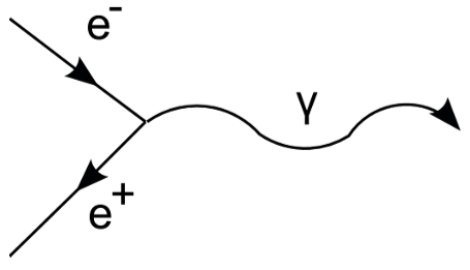
\includegraphics[scale=0.15]{./../Pictures/fig9_1.png}
    \figcaption{过程$e^+e^-\to \gamma$的Feynman图}
    \label{fig9.1}
}}
定性来说,这一项对产生一个动量$k'$光子态$\langle \gamma|$的散射振幅有贡献
\begin{gather}\label{equ9.74}
\langle f|S^{(1)}_1|i\rangle = \langle \gamma_{k'}|S^{(1)}_1|e^+(p_1),e^-(p_2)\rangle\\
=\int_{-\infty}^\infty d^4x\langle\gamma_{k'}|\sum_k\text{constant}(k)|\gamma_k\rangle \text{e}^{-ix(p_1+p_2-k)}\nonumber\\
=\int_{-\infty}^\infty d^4x\sum_k\text{constant}(k)\underbrace{\langle\gamma_{k'}||\gamma_k\rangle}_{\delta_{kk'}} \text{e}^{-ix(p_1+p_2-k)}\nonumber\\
=\int_{-\infty}^{\infty} d^4x \text{constant}(k')\text{e}^{-ix(p_1+p_2-k)}\nonumber
\end{gather}
对$x$积分导致delta函数$\delta(p_1+p_2-k)$,它代表了动量守恒条件\mpar{$e^-$的4-动量(=能量$p_0=E$与通常动量$p_i$)与$e^+$的4-动量之和,必须等于光子$\gamma$4-动量:$p_1+p_2-k\stackrel{!}{=}0$。否则由附录D.2中的解释,有$\delta(p_1+p_2-k)=0$。}。实验中无法测量、制备确定动量的粒子,真实动量总处于一个范围内。因此在计算的最后,应将散射振幅对相应的动量范围积分。

注意到其它七项对$\hat{S}^(1)$贡献为0,因为他们湮灭初态中不存在的粒子,如一个光子。若选取其它初态,如一个光子和一个正电子$|\gamma,e^+\rangle$,那么第一项贡献将为0,其余项则非0。

下面我们定性考察$\hat{S}$级数展开的第三项。
\begin{align}\label{equ9.75}
S^{(2)}&=-\frac{1}{2!}T\left\{ \left( \int_{-\infty}^\infty d^4x_1\mathscr{H}_I(x_1)\right)\left( \int_{-\infty}^\infty d^4x_2\mathscr{H}_I(x_2)\right)\right\}\nonumber\\
&=-\frac{1}{2!}T\left\{ \left( \int_{-\infty}^\infty d^4x_1gA_\mu(x_1)\bar{\Psi}(x_1)\gamma^\mu\Psi(x_1)\right)\left( \int_{-\infty}^\infty d^4x_2gA_\mu(x_2)\bar{\Psi}(x_2)\gamma^\mu\Psi(x_2)\right)\right\}
\end{align}
其中编时乘积可用Wick定理重写为对易子的正规序乘积之和,记为$N\{\}$。正规序意味着将所有产生算符放到左侧,湮灭算符则放到右侧。比如,$N\{aa^\dag a^\dag a\}=a^\dag a^\dag aa$。举例来说,求和中的一项是
\begin{gather*}
-\frac{1}{2!}g^2\int\int d^4x_1 d^4x_2 N\left\{ \bar{\Psi}(x_1)\gamma^\mu\Psi(x_1)[A_\mu(x_1),A_\mu(x_2)]\bar{\Psi}(x_2)\gamma^\mu\Psi(x_2)\right\}
\end{gather*}
其中对易子可由$A_\mu$的显式解求出,被称为光子传播子\mpar{传播子是量子场论中最难推导的对象之一。比如考虑标量传播子,推导的出发点是$i\Delta=\langle0|T\{\Phi(x)\Phi^\dag(y)\}|0\rangle$,即从真空中创造一个$y$处的粒子,再于$x$处令其湮灭。这可以重写为对易子$i\Delta=\langle0|[\Phi^{\dag+}(y),\Phi^-(x)]|0\rangle$。通过繁杂的数学计算可以得到$i\Delta=\frac{-i}{2\pi^3}\int\frac{d^3k}{\omega_k}\text{e}^{-ik(x-y)}$,这也是实际计算中使用的表达式。这些粗略描述有多处不完全正确,但它表达了这些数学构造的基本思想。}$[A_\mu(x_1),A_\mu(x_2)]\equiv iD_\mu(x_1-x_2)$。
展开这一项后会得到许多项,因为每一个$\Psi,\bar{\Psi}$等算符都是两项之和,现在只考虑其中一项。如果再次选择包含电子和正电子的初态,可以定性得到其中一项\mpar{我们又选择了电子和正电子碰撞时非零的一项}的表达式,如下所示:
\begin{align}\label{equ9.76}
-\frac{1}{2!}g^2\int\int d^4x_1 d^4x_2 \bar{\Psi}^-(x_1)\Psi^-(x_1)D_\mu(x_1-x_2)\bar{\Psi}^+(x_2)\Psi^+(x_2)|e^+,e^-\rangle
\end{align}
这可以从物理角度加以理解:
\begin{itemize}
\item 初态中的两个粒子在$x_2$处被$\bar{\Psi}^+(x_2)\Psi^+(x_2)$湮灭。
\item 之后传播子在$x_2$处产生一个“虚”光子,虚光子传播到$x_1$湮灭。
\item 最后$\bar{\Psi}^-(x_1)\Psi^-(x_1)$再次于$x_1$处产生一个电子和一个正电子。
\end{itemize}
通过这一项可以计算出反应$e^+e^-\to e^+ e^-$的概率幅,其中入射和岀射粒子的动量当然可以完全不同,但总动量保持守恒。所有其它项也同样可以诠释为有质量\mpar{此处是电子和正电子。其它可能性也包括夸克和另两种轻子$\mu$和$\tau$。}自旋$\frac{1}{2}$场和无质量\mpar{此处为光子}自旋$0$场。
{\marginpar{
    \centering
    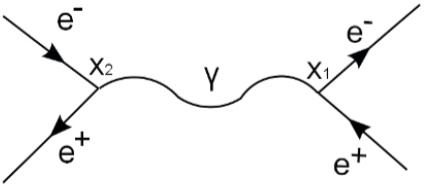
\includegraphics[scale=0.15]{./../Pictures/fig9_2.png}
    \figcaption{过程$e^+e^-\to \gamma\to e^+e^-$的Feynman图}
    \label{fig9.2}
}}

计算中得到的这类概率幅可以直接在实验中加以检验,因为概率幅直接联系于实验可测量量:散射截面。

本章描述的技术可以用于推导量子场论中的许多重要结果。之前导出的其它相互作用项也可被加入相互作用哈密顿量,而后对应的概率幅也可类似求出。不行的是,针对$\mathcal{SU}(3)$规范对称性导致的相互作用项,这一思路并不总是有效,因为强相互作用的耦合常数过大,以致无法用级数展开加以计算。若耦合常数大于1,高阶项大于低阶项,便不能用级数的前几项近似级数和。这一物理学分支被称为量子色动力学,在这门学科中需要用到其他计算方案,超出了本书讨论的范围。

\section*{Further Reading Tips 进一步的阅读建议}
\begin{itemize}
\item \textbf{Robert D. Klauber - 简明量子场论(Student Friendly Quantum Field Theory)\mpar{Robert D. Klauber. Student Friendly Quantum Field Theory. Sandtrove
Press, 2nd edition, 12 2013. ISBN
9780984513956}}按我谦逊的观点看,是最好的量子场论导论教材。所有章节都极富教学技巧,因为作者曾花费许多时间考虑读者学习量子场论时的难点。
\item \textbf{Francis Halzen, Alan D. Martin - 夸克与轻子:现代粒子物理学导论(Quarks and Leptons: An Introductory Course in Modern Particle Physics)\mpar{Francis Halzen and Alan D. Martin. Quarks and Leptons: An Introductory
Course in Modern Particle Physics. Wiley,
1st edition, 1 1984. ISBN 9780471887416}}是一本聚焦于应用量子场论计算方案的极佳之作。
\item \textbf{Anthony Zee - 果壳中的量子场论(Quantum Field Theory in a Nutshell)\mpar{Anthony Zee. Quantum Field Theory in
a Nutshell. Princeton University Press,
1st edition, 3 2003. ISBN 9780691010199}}包含许多独具匠心的论述。不过有些章节太短,初学者很难理解。对用其它书籍学过量子场论的读者,这本书十分值得一读。
\item \textbf{Franz Mandl, Graham Shaw - 量子场论(Quantum Field Theory)\mpar{Franz Mandl and Graham Shaw. Quantum Field Theory. Wiley, 2nd
edition, 5 2010. ISBN 9780471496847}}是学习弱、强相互作用理论的绝佳起点。
\item \textbf{Michele Maggiore - 量子场论现代导引(A Modern Introduction to Quantum Field Theory)\mpar{Michele Maggiore. A Modern Introduction to Quantum Field Theory. Oxford
University Press, 1st edition, 2 2005.
ISBN 9780198520740}}是一本极好的导论书籍,着重讨论了场论中的群论概念。
\item \textbf{Ian J. R. Aitchison and Anthony J. G. Hey - 粒子物理学中的规范场论(Gauge Theories in
Particle Physics)\mpar{Ian J.R. Aitchison and Anthony J.G.
Hey. Gauge Theories in Particle Physics.
CRC Press, 4th edition, 12 2012. ISBN
9781466513174}}非常清晰地诠释了规范场论的思想。
\end{itemize}

\section[Klein-Gordon 方程的一般解]{Appendix: Most General Solution of the Klein-Gordon Equation Klein-Gordon 方程的一般解}\label{sec9.6}
不难得到Klein-Gordon方程的\textbf{一个解}:平面波即满足方程。
\begin{gather*}
\Phi(x)=a\text{e}^{i(px-Et)}=\text{e}^{-ip_\mu x^\mu}
\end{gather*}
由狭义相对论能量-动量关系可得:
\begin{gather*}
E^2=\vec{p}^2+m^2\to p_\mu p^\mu=m^2
\end{gather*}
于是有
\begin{align}
(\partial_\mu\partial^\mu+m^2)\Phi&=(\partial_\mu\partial^\mu+m^2)\text{e}^{-ip_\mu x^\mu}\\
&=(-p_\mu p^\mu+m^2)\text{e}^{-ip_\mu x^\mu}\\
&=(-m^2+m^2)\text{e}^{-ip_\mu x^\mu}\\
&=0\quad\checkmark
\end{align}
由于推导中对场求导两次,指数中的符号不会影响最终结果。因而,
\begin{gather*}
\Phi^\dag(x)=a^\dag \text{e}^{-i(px-Et)}=a^\dag \text{e}^{ip_\mu x^\mu}
\end{gather*}
也是方程的解。将以上两解线性叠加,可以得到更多解。一般解由所有可能解得叠加得出,亦可写为解的Fourier展开\mpar{这便是$2\pi$因子的来源。同时,这也是解构成正交集的条件:$\int dk \text{e}^{ikx}\text{e}^{-ikx'}=\int dk \text{e}^{ik(x-x')}=2\pi\delta(x-x')$。于是$2\pi$因子即为归一化常数。}
\begin{gather*}
\Phi(x)=\int \frac{dp^4}{(2\pi)^4}(a(p)\text{e}^{-i(p_\mu x^\mu)}+a^\dag(p)\text{e}^{i(p_\mu x^\mu)})
\end{gather*}
注意到$a=a(p)$,因为不同$p$值可以对应不同的乘积因子,求和中每一项都是各自独立的解。

在文献中,波数$k_i=\frac{p_i}{\hbar}$和频率$k_0=w=\frac{E}{\hbar}$常被用以代替能量和动量。由于我们使用单位制$\hbar=1$,只需将上面公式中的变量重新命名,即可得到标准教科书中的表达式。同时,缩写$kx\equiv k_\mu x^\mu$也很常用。于是可以写出
\begin{gather*}
\Phi(x)=\int \frac{dk^4}{(2\pi)^4}\left(a(k)\text{e}^{-i(kx)}+a^\dag(k)\text{e}^{i(kx)}\right)
\end{gather*}
注意到并非所有Klein-Gordon方程的解都适用于描述自然,因为需满足\textbf{“质壳”条件(``mass-shell" condition)}
\begin{align}
p_\mu p^\mu=k_\mu k^\mu=m^2\to k_0^2-k_i^2\stackrel{!}{=}m^2\to k^2\stackrel{!}{=}m^2
\end{align}
只有满足质壳条件的解才与相对论能量-动量关系相协调(方程\eqref{equ8.2})。通过插入delta分布排除非物理(不在壳)解后\mpar{解释见附录 D. 2},这一条件可被纳入上面的方程中。
\begin{gather*}
\Phi(x)_\text{physical}=\int\frac{dk^4}{(2\pi)^4}2\pi\delta(k^2-m^2)\left(a(k)\text{e}^{-i(kx)}+a^\dag(k)\text{e}^{i(kx)}\right)
\end{gather*}
除此之外,只有正能解有物理意义,原因前面已经提到过,否则能量没有下限、系统无法处于稳定态。利用Heavside函数$\theta(k_0)$($k_0<0$时为0,$k_0\ge0$时为1)可将这一约束纳入方程。方程中的积分变为:
\begin{gather*}
\Phi(x)_\text{physical}=\int \frac{1}{(2\pi)^3}\underbrace{dk^4\delta(k^2-m^2)\theta(k_0)}_{\text{测度}}\left(a(k)\text{e}^{-i(kx)}+a^\dag(k)\text{e}^{i(kx)}\right)
\end{gather*}
等式中的测度可以重写为
\begin{align}
dk^4\delta(k^2-m^2)\theta(k_0)&=dk^4\delta(k_0^2-\vec{k}^2-m^2)\theta(k_0)
\nonumber\\
&=dk^4\delta(k_0^2-\omega_k^2)\theta(k_0)\nonumber\\
&=dk^4\delta\left((k_0-\omega_k)(k_0+\omega_k)\right)\theta(k_0)
\nonumber\\
&\underbrace{=}_{\mathclap{\text{使用}\delta\left(f(x)\right)=\sum_i\frac{\delta(x-a_i)}{\left|\frac{df}{dx}(a_i)\right|}\text{,其中}a_i{为函数f的根,即}f(a_i)=0}}dk^4\frac{1}{2k_0}\left(\delta(k_0-\omega_k)+\delta(k_0+\omega_k)\right)\theta(k_0)\nonumber\\
&\underbrace{=}_{\mathclap{\text{因为}\delta(k_0+\omega_k\text{的参数在}k_0\ge0\text{时永不为0}}}dk^4\frac{1}{k_0}\delta(k_0-\omega_k)\nonumber\\
&=dk^3dk_0\frac{1}{2k_0}\delta(k_0-\omega_k)\nonumber\\
&\underbrace{=}_{\text{对}k_0\text{积分}}dk^3\frac{1}{2\omega_k}
\end{align}
最终得到满足物理条件的Klein-Gordon方程一般解
\begin{align}
\Phi(x)=\int dk^3\frac{1}{(2\pi)^32\omega_k}\left(a(k)\text{e}^{-i(kx)}+a^\dag(k)\text{e}^{i(kx)}\right)
\end{align}







